% Springer Nature journal article template, configured for Nature Portfolio style.
\documentclass[pdflatex,sn-nature]{sn-jnl}

\usepackage{graphicx}%
\usepackage{multirow}%
\usepackage{amsmath,amssymb,amsfonts}%
\usepackage{bm}%
\usepackage{xcolor}%
\usepackage{textcomp}%
\usepackage{booktabs}%
\usepackage{tikz}%
\usetikzlibrary{arrows.meta,positioning,fit}

\graphicspath{{./}}

\newcommand{\vect}[1]{\bm{#1}}
\newcommand{\E}{\mathbb{E}}
\newcommand{\CN}{\mathcal{CN}}
\newcommand{\Jobj}{\mathcal{J}}

\begin{document}

\title[Adaptive metasurfaces for 6G healthcare]{Morphology-Adaptive Stacked Intelligent Metasurfaces for Contactless Cardiopulmonary Radar Monitoring for 6G Healthcare}

\author*[1]{\fnm{Shuja} \sur{Ansari}}\email{shuja.ansari@uaeu.ac.ae}
\author[1]{\fnm{Oguzhan} \sur{Akgol}}
\author[2]{\fnm{Qammer} \sur{Abbasi}}
\author[1]{\fnm{Hammad} \sur{Al Khoori}}

\affil*[1]{\orgdiv{Department of Electrical and Communications Engineering, College of Engineering},
\orgname{United Arab Emirates University},
\orgaddress{\city{Al Ain}, \country{UAE}}}

\affil[2]{\orgdiv{James Watt School of Engineering},
\orgname{University of Glasgow},
\orgaddress{\city{Glasgow}, \country{United Kingdom}}}

\abstract{
Contactless radar can recover respiration and heartbeat from chest-wall micromotion,
but the weak cardiac component is vulnerable to multipath, nearby motion and
morphology-dependent scattering. We propose a morphology-adaptive stacked intelligent
metasurface (SIM) that performs phase-only processing of the reflected field before a
single detector. Programmable phase masks are interleaved with Fresnel coupling
operators and optimized with an exact electromagnetic adjoint gradient, forming a
linear wave-domain neural processor. Body mass index (BMI) is an observable
conditioning variable for a parametric morphology surrogate, not a clinical law. A
reproducible 30-GHz digital twin compares single-antenna, 36-channel digital-array,
one-layer surface, universal three-layer SIM and BMI-adaptive three-layer SIM
receivers. At 8-dB reference signal-to-noise ratio, the adaptive SIM attains 9.29-dB
mean spatial signal-to-interference-plus-noise ratio, versus 9.32 dB for the digital
array, 8.38 dB for the universal SIM, 5.72 dB for the one-layer surface and $-9.90$
dB for a single antenna. Its respiration- and heart-rate root-mean-square errors are
0.05 breaths/min and 0.08 beats/min. Six-bit phase control approaches continuous
control, while two layers maximize the tested SINR with 0.5-dB loss per layer. These
findings are a testable system hypothesis, not clinical or full-wave hardware
validation.
}

\keywords{
6G healthcare, contactless vital-sign monitoring, Doppler radar, electromagnetic
neural network, stacked intelligent metasurface, wave-domain processing
}

\maketitle

\section{Introduction}
Radar is attractive for physiological monitoring because it senses motion without
requiring an electrode, chest strap or wearable device. Continuous-wave (CW),
frequency-modulated continuous-wave (FMCW) and ultra-wideband systems have all been
used to recover breathing and cardiac activity \cite{li2013review,hu2014quadrature,
michler2019clinical}. Detecting a person, however, is much easier than recovering a
stable heartbeat waveform. In a quiet measurement the respiratory displacement is
usually dominant. Its harmonics, small posture changes, random body motion and I/Q
offsets can obscure the weaker cardiac component \cite{li2008movement,li2013review}.
This remains a practical difficulty outside tightly controlled laboratory settings.
A postoperative FMCW study, for example, obtained better respiratory agreement after
movement-contaminated intervals were removed, but reported poorer accuracy during
spontaneous breathing \cite{vanloon2016clinical}.

Spatial processing can help when the chest return and unwanted motion arrive from
different directions. The conventional solution is a digital antenna array, which is
flexible but requires a receiver and data-conversion path for each spatial channel.
For a compact 6G healthcare sensor, that hardware cost may be difficult to justify.
Our interest is therefore in moving part of the spatial processing in front of the
receiver, where the electromagnetic field itself can be shaped before it is sampled.

A stacked intelligent metasurface (SIM) provides one possible route. Its programmable
layers are separated by free-space regions, so phase modulation at one layer is mixed
by diffraction before reaching the next. This cascaded operation has been studied for
wave-domain beamforming, interference suppression and sensing
\cite{an2023beamforming,an2024transceiver,an2024dft,niu2024isac}. The idea is closely
related to diffractive neural processors demonstrated at optical and microwave
frequencies \cite{lin2018d2nn,liu2022programmable}. We use the neural-network analogy
only in this limited sense: the phase states are trainable and the intervening
propagation couples the elements. A passive narrowband stack is still a linear
complex-field operator; it does not contain a physical nonlinear activation.

An additional issue is that the desired field need not be identical for every
person. Measurement position and subject anatomy affect radar signal quality, as is
also evident in public synchronized datasets \cite{shi2020dataset,edanami2022dataset}.
We use body mass index (BMI) as a readily available conditioning variable, while
recognizing that BMI is only a coarse proxy for body morphology. It cannot determine
tissue permittivity, fat distribution, thoracic geometry or radar cross section on
its own. The BMI-dependent relations introduced below are therefore transparent
simulation assumptions that can later be replaced by full-wave or measured data.

Against this background, we ask a narrow system question: if morphology changes the
spatial signature of the thoracic return, can a morphology-conditioned SIM retain
cardiopulmonary micromotion while suppressing spatially distinct moving clutter more
effectively than a single universal phase stack? We examine this question with a
coupled physiological--electromagnetic digital twin and an exact adjoint gradient for
phase-only optimization. The adaptive stack is compared with a single antenna, a
36-channel robust digital array, a one-layer intelligent surface and a universal
three-layer SIM under paired Monte Carlo trials. We then vary the receiver SNR, phase
resolution, layer loss and BMI-codebook error. The purpose is to establish a
reproducible engineering hypothesis and its limits, rather than to claim clinical
performance from synthetic data.

\section{System and Signal Model}

\subsection{Architecture}
Figure~\ref{fig:architecture} summarizes the receive chain considered here. The
illuminating radar is conventional; the change is on reception, where the thoracic
return and the nuisance fields encounter the SIM before reaching a single detector.
We assume that the controller selects an offline-optimized phase stack from a
BMI-indexed codebook. The BMI value is entered during setup or obtained from an
existing record. Estimating it from the radar signal is outside the present model.

\begin{figure}[htbp]
\centering
\resizebox{0.98\linewidth}{!}{%
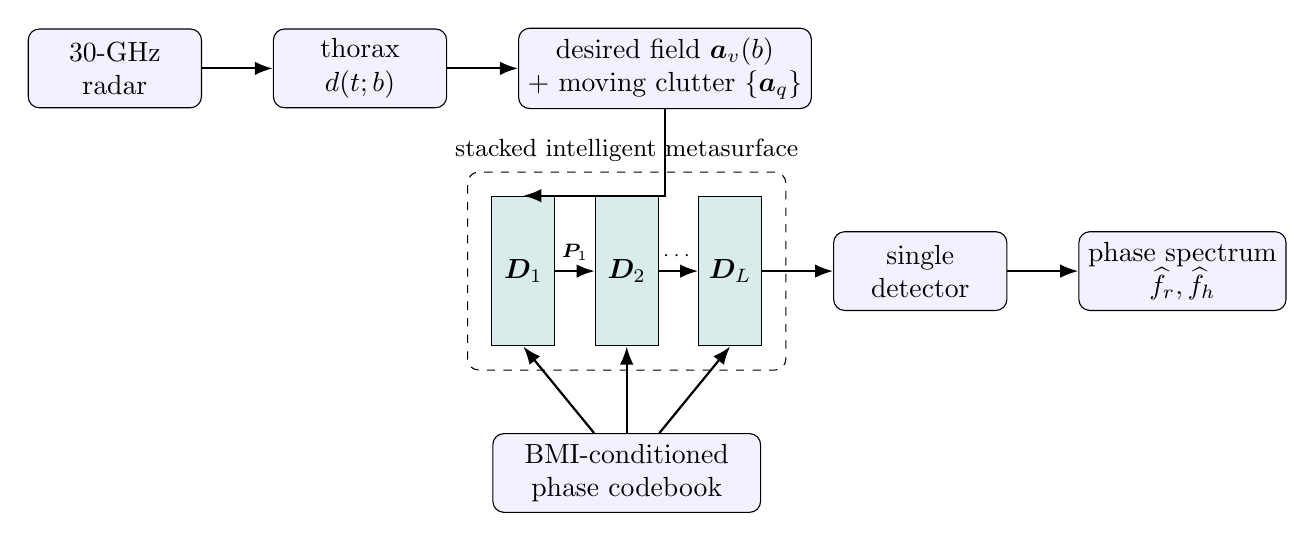
\begin{tikzpicture}[
    node distance=11mm and 9mm,
    block/.style={draw, rounded corners, minimum height=10mm, minimum width=22mm,
                  align=center, fill=blue!5},
    surface/.style={draw, minimum height=19mm, minimum width=8mm, fill=teal!15},
    arrow/.style={-{Latex[length=2.3mm]}, thick}
]
\node[block] (radar) {30-GHz\\radar};
\node[block, right=of radar] (subject) {thorax\\$d(t;b)$};
\node[block, right=of subject, minimum width=37mm] (field) {desired field $\vect a_v(b)$\\+ moving clutter $\{\vect a_q\}$};
\node[surface, below=of field, xshift=-18mm] (l1) {$\vect D_1$};
\node[surface, right=5mm of l1] (l2) {$\vect D_2$};
\node[surface, right=5mm of l2] (l3) {$\vect D_L$};
\node[block, right=of l3] (rx) {single\\detector};
\node[block, right=of rx] (est) {phase spectrum\\$\widehat f_r,\widehat f_h$};
\node[block, below=11mm of l2, minimum width=34mm] (control) {BMI-conditioned\\phase codebook};
\draw[arrow] (radar) -- (subject);
\draw[arrow] (subject) -- (field);
\draw[arrow] (field.south) |- (l1.north);
\draw[arrow] (l1) -- node[above, font=\scriptsize] {$\vect P_1$} (l2);
\draw[arrow] (l2) -- node[above, font=\scriptsize] {$\cdots$} (l3);
\draw[arrow] (l3) -- (rx);
\draw[arrow] (rx) -- (est);
\draw[arrow] (control) -- (l1.south);
\draw[arrow] (control) -- (l2.south);
\draw[arrow] (control) -- (l3.south);
\node[draw, dashed, rounded corners, fit=(l1)(l2)(l3), inner sep=3mm,
      label=above:{\small stacked intelligent metasurface}] {};
\end{tikzpicture}
}
\caption{Proposed morphology-adaptive wave-domain receiver. The phase masks are
optimized offline. During sensing, BMI selects a codebook entry and the reflected
field is transformed electromagnetically before a single detector.}
\label{fig:architecture}
\end{figure}

\subsection{Physiological phase modulation}
Let $b$ denote the BMI value used for conditioning. We represent anterior chest-wall
motion by the sum of respiratory and cardiac components,
\begin{equation}
\begin{aligned}
d(t;b)={}&A_r(b)\sin\!\left(2\pi f_r t+\phi_r(t)\right)\\
&+A_h(b)\sin\!\left(2\pi f_h t+\phi_h(t)\right),
\end{aligned}
\label{eq:displacement}
\end{equation}
where $f_r$ and $f_h$ are the respiration and heartbeat frequencies. Slowly varying
terms in $\phi_r(t)$ and $\phi_h(t)$ prevent the simulated waveform from being
perfectly periodic. At wavelength $\lambda=c/f_c$, the corresponding narrowband
return is
\begin{equation}
s_v(t;b)=\alpha(b)\exp\!\left(j\frac{4\pi}{\lambda}d(t;b)\right).
\label{eq:vitalreturn}
\end{equation}
where the factor $4\pi/\lambda$ accounts for the two-way path. We deliberately use
simple exponential maps for the morphology dependence,
\begin{align}
\alpha(b)&=\exp[-0.035\max(b-22,0)],\label{eq:alpha}\\
A_r(b)&=4.0\,\mathrm{mm}\,\exp[-0.012\max(b-22,0)],\label{eq:ar}\\
A_h(b)&=0.24\,\mathrm{mm}\,\exp[-0.020\max(b-22,0)].\label{eq:ah}
\end{align}
These functions are not fitted population relationships. Their role is to create a
controlled reduction in return strength and micromotion amplitude across the test
range. Keeping them explicit makes it straightforward to replace them when measured
or full-wave data become available.

\subsection{BMI-conditioned spatial signature}
For aperture steering vector $\vect a(\Omega)$, the desired first-layer field is a
coherent mixture of a central and two diffuse components:
\begin{equation}
\begin{aligned}
\vect a_v(b)=\frac{1}{C_b}\Big[\,&(1-\rho_b)\vect a(\Omega_0(b))\\
&+0.55\rho_b e^{j\psi_b}\vect a(\Omega_-(b))\\
&+0.45\rho_b e^{-j0.7\psi_b}\vect a(\Omega_+(b))\Big]
\odot\vect c_b,
\end{aligned}
\label{eq:morphology}
\end{equation}
Here, $C_b$ normalizes the field, $\rho_b$ sets the diffuse fraction and $\vect c_b$
introduces quadratic phase curvature to mimic a change in effective scattering depth.
Independent angular jitter is used during training and testing. This spatial model is
important. If the desired return and the clutter were represented by a common scalar
phase alone, no static passive linear surface could separate them.

\subsection{Multilayer wave-domain transformation}
The $N$ elements of layer $\ell$ implement
\begin{equation}
\begin{aligned}
\vect D_\ell(\vect\theta_\ell)
=\operatorname{diag}\!\big(&e^{j\theta_{\ell,1}},\ldots,\\
&e^{j\theta_{\ell,N}}\big).
\end{aligned}
\end{equation}
For element positions $(x_n,y_n)$ and layer spacing $z_\ell$, scalar Green-function
coupling is sampled as
\begin{equation}
\begin{aligned}
[\widetilde{\vect P}_\ell]_{mn}
&=\frac{\exp(jkr_{mn})}{r_{mn}},\\
r_{mn}&=\sqrt{(x_m-x_n)^2+(y_m-y_n)^2+z_\ell^2}.
\end{aligned}
\label{eq:green}
\end{equation}
We do not assume a particular fabricated unit cell at this stage. Instead, the finite
coupling matrix is projected onto its closest unitary polar factor
$\vect P_\ell=\vect U_\ell\vect V_\ell^H$, where
$\widetilde{\vect P}_\ell=\vect U_\ell\vect\Sigma_\ell\vect V_\ell^H$. This retains
the Fresnel-like modal mixing while allowing insertion loss to be introduced
separately. With field transmission $\eta_\ell$, the layer recursion becomes
\begin{equation}
\begin{aligned}
\vect u_{\ell+1}&=\eta_\ell\vect P_\ell\vect D_\ell\vect u_\ell,\\
\eta_\ell&=10^{-\xi_\ell/20},
\end{aligned}
\label{eq:forward}
\end{equation}
where $\xi_\ell$ denotes the loss assigned to layer $\ell$ in decibels. For output
mode $\vect w$, source $q$ then has the effective gain
\begin{equation}
\begin{aligned}
g_q(\vect\Theta)=\vect w^H
&\left(\eta_L\vect P_L\vect D_L\right)\cdots\\
&\left(\eta_1\vect P_1\vect D_1\right)\vect a_q.
\end{aligned}
\label{eq:gain}
\end{equation}

\subsection{Detector signal}
With $Q$ moving nuisance reflectors,
\begin{equation}
\begin{aligned}
y(t;b)={}&g_v(\vect\Theta,b)s_v(t;b)\\
&+\sum_{q=1}^{Q}\sqrt{p_q}\,g_q(\vect\Theta)c_q(t)+n(t),
\end{aligned}
\label{eq:received}
\end{equation}
where $n(t)\sim\CN(0,\sigma_n^2)$. We include nuisance motion both inside and outside
the two vital-sign bands. Removing the temporal mean represents the usual static
clutter and I/Q-centre calibration; the time-varying part of each nuisance return is
left intact.

\section{Adaptive SIM Optimization}

\subsection{Mean log-SINR objective}
The phase masks should strengthen the thoracic field without simply amplifying the
moving clutter. For a training set $\mathcal B$ of morphology conditions, we define
\begin{equation}
\begin{aligned}
S_b&=\alpha^2(b)|g_v(\vect\Theta,b)|^2,\\
I&=\sum_{q=1}^{Q}p_q|g_q(\vect\Theta)|^2+\sigma_0^2.
\end{aligned}
\end{equation}
and optimize
\begin{equation}
\begin{aligned}
\max_{\vect\Theta}\quad
\Jobj(\vect\Theta)&=\frac{1}{|\mathcal B|}
\sum_{b\in\mathcal B}\log S_b-\log I,\\
\text{subject to}\quad&\theta_{\ell,n}\in[-\pi,\pi).
\end{aligned}
\label{eq:objective}
\end{equation}
For the universal design, $\mathcal B$ contains the complete BMI grid and only one
stack is trained. For the adaptive design, we optimize a separate
$\vect\Theta_b$ for every codebook entry and use the nearest entry during sensing.
The logarithmic objective was chosen so that conditions with a naturally stronger
return do not dominate the universal solution.

\subsection{Electromagnetic adjoint gradient}
Let $\vect v_\ell=\vect D_\ell\vect u_\ell$. Starting from the detector mode, define
\begin{equation}
\begin{aligned}
\vect r_\ell&=(\eta_\ell\vect P_\ell)^H\vect q_{\ell+1},\\
\vect q_\ell&=\vect D_\ell^H\vect r_\ell.
\end{aligned}
\end{equation}
The exact real phase derivative for one source is
\begin{equation}
\begin{aligned}
\frac{\partial |g|^2}{\partial\theta_{\ell,n}}
=2\operatorname{Re}\!\left\{g^*jv_{\ell,n}r_{\ell,n}^*\right\}.
\end{aligned}
\label{eq:gradient}
\end{equation}
The target and clutter terms are combined through the chain rule for
Eq.~\eqref{eq:objective}. We use Adam \cite{kingma2015adam} for phase ascent and wrap
the result into $[-\pi,\pi)$ after every update. Before running the main experiments,
we checked the adjoint derivative against a central finite-difference calculation.

\subsection{Hardware-constrained masks}
For $B$ phase-control bits, continuous coefficients are quantized after training:
\begin{equation}
\begin{aligned}
\widehat\theta_{\ell,n}^{(B)}&=\Delta_B
\left\lfloor\frac{\theta_{\ell,n}}{\Delta_B}+\frac12\right\rfloor
\bmod 2\pi,\\
\Delta_B&=\frac{2\pi}{2^B}.
\end{aligned}
\label{eq:quantization}
\end{equation}
We apply this rule after continuous-phase training. The resulting experiment therefore
measures the penalty of direct hardware quantization; it does not include
quantization-aware retraining.

\section{Baselines and Rate Estimation}

We compare five receivers under the same simulated scenes.
\begin{enumerate}
    \item \textbf{Single antenna:} one central aperture sample and no intelligent
    spatial processing.
    \item \textbf{Digital robust MVDR-family array:} a unit-norm complex combiner
    with one receiver channel per aperture element \cite{capon1969mvdr}.
    \item \textbf{One-layer adaptive RIS:} one BMI-conditioned phase mask and one
    detector.
    \item \textbf{Universal three-layer SIM:} one mask stack trained over all BMI
    conditions.
    \item \textbf{Adaptive three-layer SIM:} a nearest-BMI phase-codebook stack.
\end{enumerate}

For the digital baseline, the nuisance and robust target covariances are
\begin{align}
\vect R_i&=\sum_q p_q\vect a_q\vect a_q^H+\sigma_0^2\vect I,\\
\vect R_s(b)&=\frac{1}{M}\sum_{m=1}^{M}
\vect a_{v,m}(b)\vect a_{v,m}^H(b).
\end{align}
The dominant generalized eigenvector of
$\vect R_s\vect w=\lambda\vect R_i\vect w$ provides the initial combiner. We then
refine it on the complex unit sphere using the same mean log-SINR objective as the
SIM. This is intentionally a demanding reference: it has access to all 36 complex
spatial channels, whereas each surface-based receiver terminates in one detector.

Rate estimation is kept deliberately simple so that differences are driven mainly by
the spatial front end. We unwrap and linearly detrend the received phase, apply a Hann
window, and calculate an eightfold zero-padded FFT. Quadratic interpolation of the
log-spectrum gives the largest peak in 0.10--0.60 Hz for respiration and
0.80--2.20 Hz for heartbeat. Across $K$ trials, the rate error is
\begin{equation}
\begin{aligned}
\operatorname{RMSE}_x
&=60\sqrt{\frac{1}{K}\sum_{k=1}^{K}
(\widehat f_{x,k}-f_{x,k})^2},\\
&\hspace{22mm}x\in\{r,h\}.
\end{aligned}
\label{eq:rmse}
\end{equation}

\section{Methods}

The reference configuration is collected in Table~\ref{tab:parameters}. We fixed the
random seed at 2026 and used paired trials: every receiver sees the same physiological
frequencies, spatial jitter, nuisance phases and normalized noise realization. This
removes scene-to-scene variation from comparisons between receivers. The reference
SNR $\gamma$ is defined using the desired power at one aperture element,
\begin{equation}
\sigma_n^2=\frac{\alpha^2(b)}{N}10^{-\gamma/10}.
\label{eq:noise}
\end{equation}
so aperture gain can emerge from coherent collection without multiplying the noise
power by the number of metasurface elements.

\begin{table}[t]
\caption{Reference simulation parameters}
\label{tab:parameters}
\centering
\footnotesize
\begin{tabular}{ll}
\toprule
Parameter & Value \\
\midrule
Carrier frequency & 30 GHz \\
Wavelength & 9.99 mm \\
SIM aperture & $6\times6$ elements ($N=36$) \\
Element pitch & 5 mm \\
Inter-layer spacing & 12 mm \\
Sampling rate / duration & 20 Hz / 30 s \\
BMI codebook & $\{18,22,26,30,34,38\}$ kg/m$^2$ \\
Respiration frequency & $\mathcal U(0.18,0.42)$ Hz \\
Heart frequency & $\mathcal U(0.95,1.65)$ Hz \\
Nuisance fields & 8 moving spatial sources \\
Training variants & 4/BMI universal; 6/BMI adaptive \\
Optimizer & Adam, 180 iterations, step 0.045 \\
Main evaluation & 10 trials per BMI at 8 dB \\
Sensitivity evaluation & 12 trials per condition \\
SNR sweep & $-10,-5,0,5,10,15$ dB \\
Phase resolution & 1, 2, 3, 4, 6 bits; continuous \\
Depth / assumed loss & 1--5 layers / 0.5 dB per layer \\
BMI-selection bias & $-8,-4,0,4,8$ kg/m$^2$ \\
\bottomrule
\end{tabular}
\end{table}

For the main five-receiver comparison, propagation between the phase masks is
lossless. This isolates the spatial degrees of freedom of each architecture. Loss is
introduced separately in the depth study at 0.5 dB per layer. We report spatial
performance as
\begin{equation}
\Gamma_b=10\log_{10}\!\left(
\frac{\alpha^2(b)|g_v|^2}
{\sum_qp_q|g_q|^2+\sigma_0^2}\right).
\label{eq:sinr}
\end{equation}
The implementation is also checked with five automated tests covering field
normalization, clean-signal rate recovery, phase quantization, codebook remapping and
the adjoint gradient.

\section{Results}

\subsection{Reference comparison}
Table~\ref{tab:mainresults} gives the mean over all six BMI conditions at the 8-dB
reference SNR. The adaptive SIM reaches 9.29 dB spatial SINR. This is 3.57 dB above
the adaptive one-layer surface and 0.91 dB above the universal three-layer stack. It
is also only 0.03 dB below the 36-channel digital array. That small difference is a
property of the ideal modal model: the layers and the output port together can realize
an effective complex spatial combiner. We do not expect this equality to survive
unchanged once measured loss, coupling, bandwidth and calibration error are included.

\begin{table}[htbp]
\caption{Reference results at 8-dB single-antenna SNR (simulation only)}
\label{tab:mainresults}
\centering
\resizebox{\linewidth}{!}{%
\begin{tabular}{lccc}
\toprule
Method & Mean spatial SINR (dB) & Respiration RMSE (breaths/min) & Heart RMSE (beats/min) \\
\midrule
No intelligent surface & $-9.90$ & 13.29 & 22.31 \\
Digital robust MVDR array (BMI-adaptive) & 9.32 & 0.05 & 1.09 \\
One-layer RIS (BMI-adaptive) & 5.72 & 0.05 & 0.16 \\
Three-layer SIM (universal) & 8.38 & 0.05 & 1.16 \\
\textbf{Three-layer SIM (BMI-adaptive)} & \textbf{9.29} & \textbf{0.05} & \textbf{0.08} \\
\bottomrule
\end{tabular}
}
\end{table}

Spatial SINR does not tell the whole story. Cardiac RMSE depends on where the residual
clutter falls in frequency, not only on its total power. In this seeded run, the
digital and universal receivers each fail at one BMI condition, while the adaptive
SIM remains stable. We regard this as a feature of the particular ensemble rather
than evidence of a general advantage; substantially more trials would be needed to
support the latter claim.

Figure~\ref{fig:bmi_sinr} separates the results by conditioning value. As the assumed
target attenuation increases, the single-antenna baseline deteriorates. The adaptive
SIM follows the digital array closely and remains above the universal stack, with the
largest separation at the lower edge of the BMI grid and around BMI 22.

\begin{figure}[htbp]
\centering
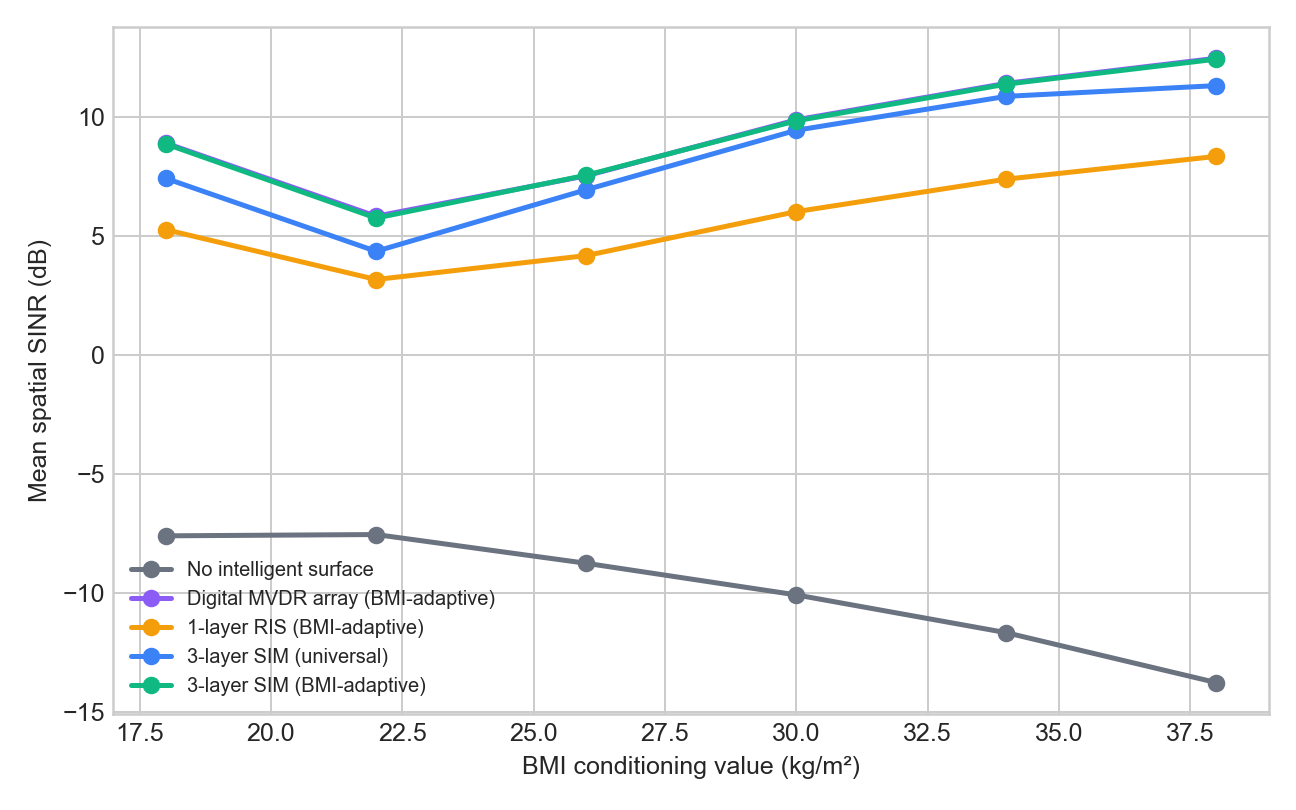
\includegraphics[width=0.96\linewidth]{spatial_sinr_vs_bmi.png}
\caption{Mean spatial SINR versus BMI conditioning value for the five receiver
architectures. The mapping from BMI to field response is parametric and unvalidated.}
\label{fig:bmi_sinr}
\end{figure}

\subsection{SNR robustness}
The SNR sweep in Fig.~\ref{fig:snr} reveals a clear operating threshold. At 0 dB,
the adaptive SIM recovers respiration reasonably well, with an RMSE of 1.62
breaths/min, but its heart-rate RMSE is still 10.26 beats/min. At 5 dB these errors
fall to 0.05 breaths/min and 0.12 beats/min. Below $-5$ dB, every receiver frequently
locks onto the wrong spectral peak. Ranking the methods by their already large errors
in that region would therefore be misleading.

\begin{figure}[htbp]
\centering
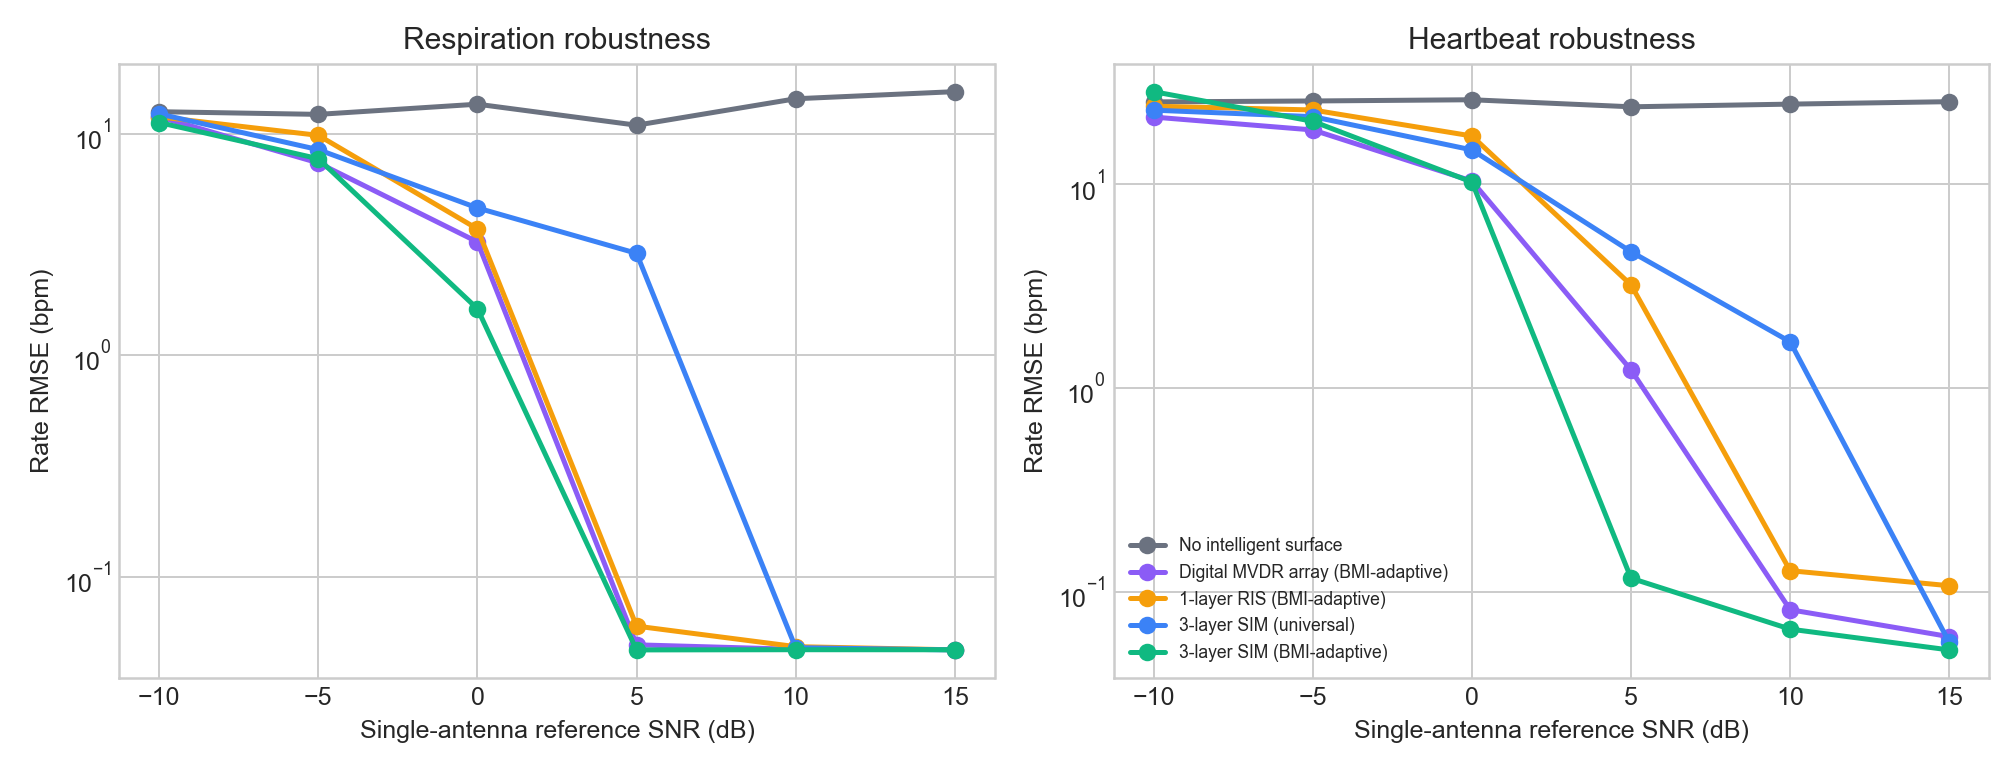
\includegraphics[width=\linewidth]{snr_robustness.png}
\caption{Rate-estimation robustness versus single-antenna reference SNR. The
logarithmic ordinate exposes the estimator transition between 0 and 5 dB.}
\label{fig:snr}
\end{figure}

\subsection{Finite phase resolution}
Directly rounding the optimized phases is costly below four bits
(Fig.~\ref{fig:quantization}). With six-bit control, the mean SINR is 9.00 dB and the
heart-rate RMSE is 0.08 beats/min, close to 9.25 dB and 0.08 beats/min for continuous
phase. Four-bit control falls to 5.70 dB and 1.91 beats/min. The one- and two-bit
points are not monotonic because coarse, independent rounding can either preserve or
remove a particular interference null by chance. Neither resolution is reliable in
this experiment.

\begin{figure}[htbp]
\centering
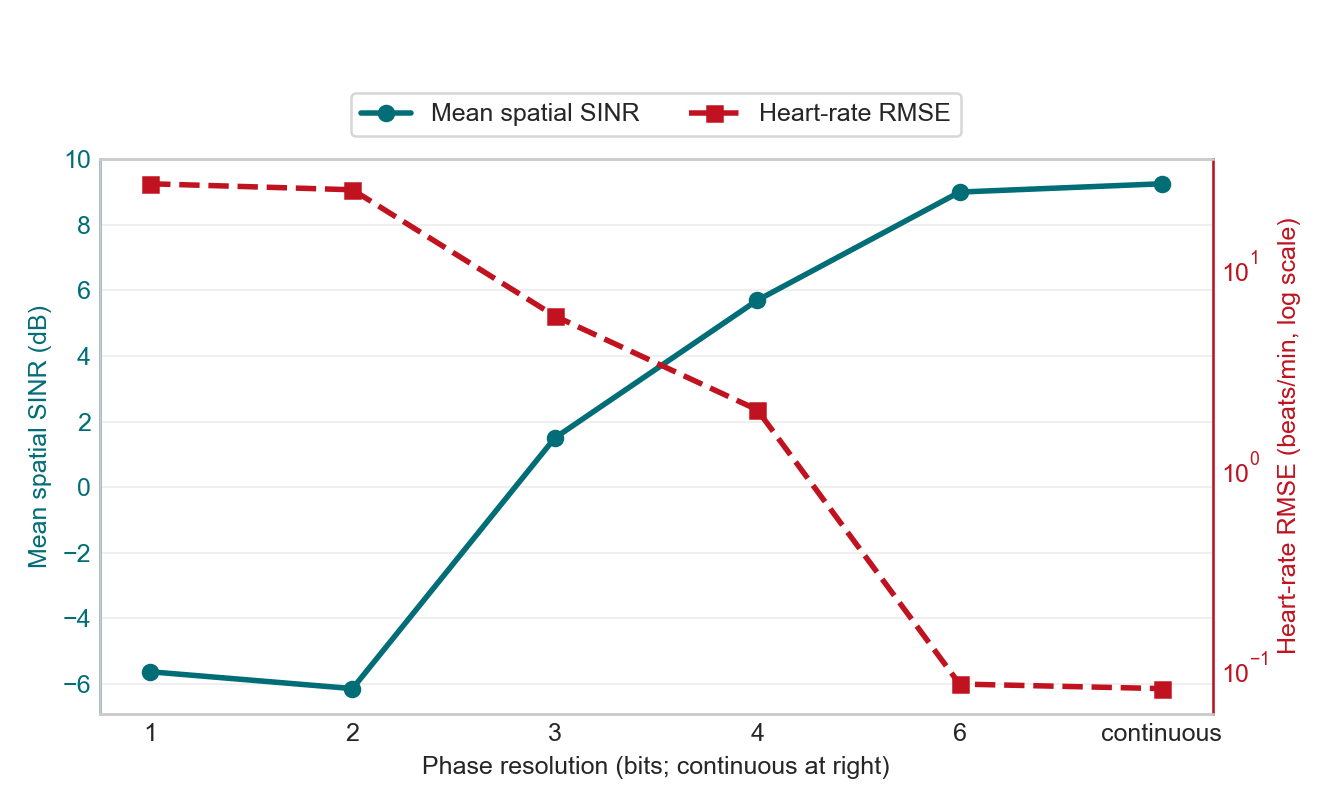
\includegraphics[width=0.98\linewidth]{phase_quantization.png}
\caption{Adaptive three-layer SIM performance after post-training phase
quantization. Mean spatial SINR uses the left axis and heart-rate RMSE uses the
logarithmic right axis. Quantization-aware retraining is not used.}
\label{fig:quantization}
\end{figure}

\subsection{Depth--loss tradeoff}
Once each layer is assigned 0.5 dB insertion loss, a deeper stack is no longer always
better. Two layers give the best point in the tested set, at 8.29 dB SINR and 0.08
beats/min heart-rate RMSE (Fig.~\ref{fig:depth}). A third layer adds controllable
phases but also another 0.5 dB loss, reducing the SINR to 8.08 dB. The location of
this optimum is tied to the assumed loss and should not be treated as a universal
two-layer rule.

\begin{figure}[htbp]
\centering
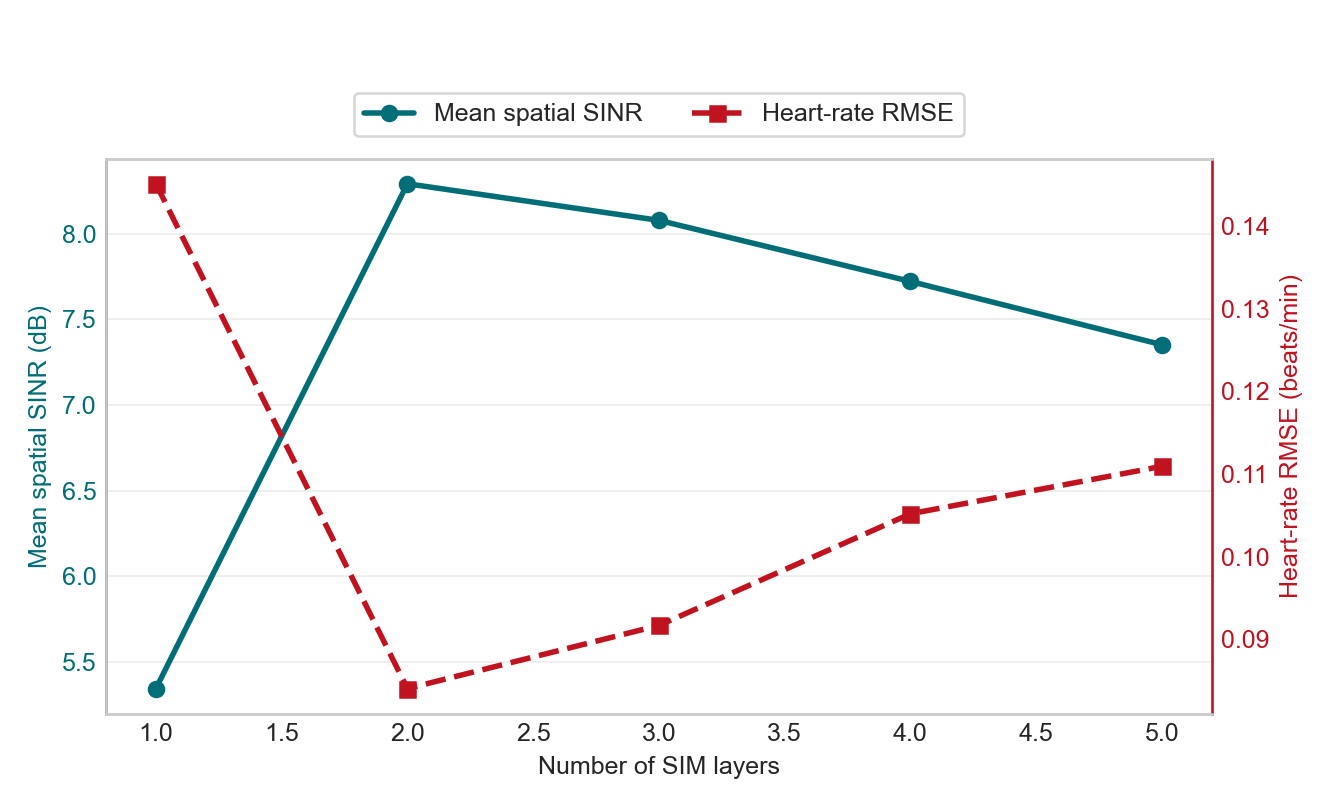
\includegraphics[width=0.96\linewidth]{layer_depth.png}
\caption{Layer-depth sensitivity with 0.5 dB insertion loss per layer. Mean
spatial SINR uses the left axis and heart-rate RMSE uses the right axis.}
\label{fig:depth}
\end{figure}

\subsection{Conditioning mismatch}
If $b$ is the simulated morphology and $\widehat b=b+\delta_b$ is supplied to the
controller, the selected code is
\begin{equation}
\begin{aligned}
c(\widehat b)&=\arg\min_{\beta\in\mathcal B_c}|\widehat b-\beta|,\\
\vect\Theta&=\vect\Theta_{c(\widehat b)}.
\end{aligned}
\end{equation}
In Fig.~\ref{fig:mismatch}, the simulated subject is held fixed and only
$\delta_b$ is changed. Selecting a code with a bias of $-8$ kg/m$^2$ costs 2.41 dB
relative to the unbiased case. A $+8$ kg/m$^2$ bias still gives 7.29 dB mean SINR,
yet the heart-rate RMSE rises to 5.89 beats/min. This is another example of residual
clutter structure mattering more than total interference power. The observed
asymmetry comes from the finite codebook and the chosen morphology map; it is not a
claim about physiological asymmetry.

\begin{figure}[htbp]
\centering
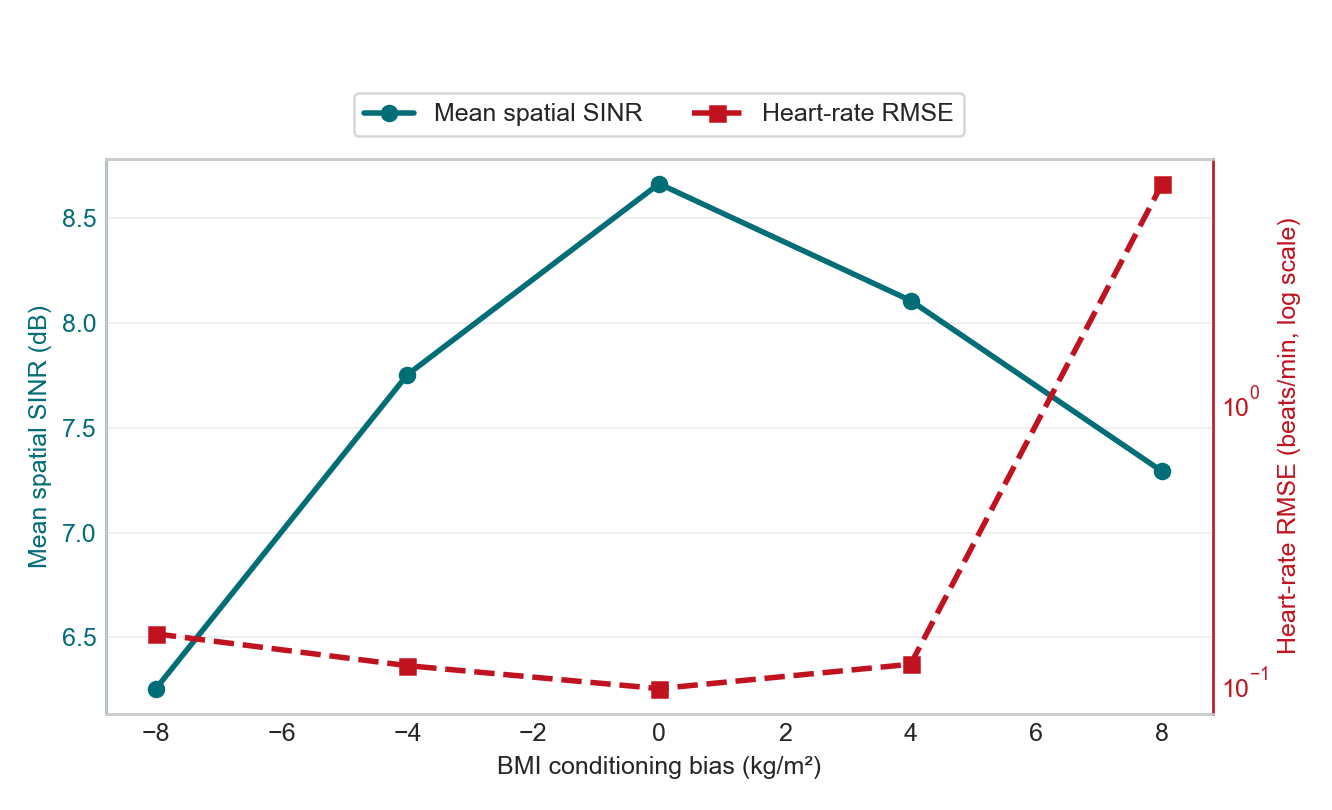
\includegraphics[width=0.96\linewidth]{bmi_mismatch.png}
\caption{Sensitivity to biased BMI codebook selection at 8-dB reference SNR.
Mean spatial SINR uses the left axis and heart-rate RMSE uses the logarithmic
right axis.}
\label{fig:mismatch}
\end{figure}

\section{Discussion}

Three observations are particularly relevant to a practical design. First, under the
single-output narrowband model, a passive stack can approach the spatial SINR of a
fully digital array while retaining one detector. The useful comparison is therefore
between RF-chain complexity and electromagnetic implementation loss, not between SIM
and unconstrained digital processing in the abstract. Second, morphology conditioning
has value only when changes in the desired field affect its separation from nearby
clutter modes. If those modes are already well separated, a universal stack is the
simpler choice. Third, hardware detail can outweigh nominal network depth. Here,
six-bit control behaves much like continuous phase, whereas accumulated loss causes
the two-layer design to outperform deeper stacks.

The word ``neural'' also needs care. Equations~\eqref{eq:forward} and
\eqref{eq:gain} describe a trainable multilayer operator, and its phases are optimized
by backpropagating an adjoint field. Its selectivity nevertheless comes from coherent
interference in a linear passive structure. The nonlinear operations occur after the
detector, in phase recovery and rate estimation.

\subsection{Limitations and required validation}
The largest uncertainty is the absence of measured, morphology-conditioned
electromagnetic data. BMI cannot resolve fat distribution, waist circumference,
posture, thoracic geometry, clothing or tissue permittivity. Equations
\eqref{eq:alpha}--\eqref{eq:morphology} should therefore be regarded as placeholders
for a relationship that still has to be measured. They would need to be calibrated
with anatomically representative phantoms or synchronized human measurements before
supporting any population-level conclusion.

The propagation model is also intentionally idealized. It omits mutual coupling,
finite-aperture edge effects, frequency dispersion, angle-dependent element response,
phase--amplitude coupling, fabrication tolerance, controller latency and thermal
drift. The scene contains one subject and simplified moving reflectors, static-clutter
calibration is assumed to be effective, and the rate estimator is deliberately basic.
The Monte Carlo ensemble demonstrates reproducibility of the code and trends; it is
not large enough to establish clinical accuracy or limits of agreement.

The immediate electromagnetic follow-up is well defined. A programmable unit cell
can be simulated over frequency, phase state, incidence angle and polarization to
obtain its complex reflection and transmission coefficients. Those data would replace
the ideal diagonal mask and the assumed scalar loss with measured or full-wave
frequency-dependent operators. A finite multilayer model could then quantify mutual
coupling, edge diffraction and the loss--depth tradeoff before a surface is fabricated.
After that calibration, the frozen designs should be tested first on phantoms, then on
public synchronized radar/ECG/respiration datasets \cite{shi2020dataset,
edanami2022dataset}, and finally in an appropriately approved human-subject study.

\section{Reproducibility}
\noindent\textbf{GitHub repository:} \url{GITHUB_REPOSITORY_URL_TO_BE_ADDED}

\section{Conclusion}
We have examined whether a stacked intelligent metasurface can adapt its receive-side
field transformation to a simple morphology condition for contactless respiration and
heartbeat sensing. Within the present digital twin, the adaptive three-layer SIM
reaches the spatial SINR of a 36-channel robust digital array to within 0.03 dB and
outperforms both a one-layer surface and a universal stack. The sensitivity studies
also expose the engineering constraints behind that result: rate recovery becomes
reliable only above the observed SNR threshold, coarse phase control is damaging, and
realistic layer loss can make a shallower stack preferable. These findings make a
case for full-wave and phantom validation, but they do not replace either. The next
step is to substitute electromagnetic S-parameters and measured morphology data for
the ideal operators used here.

\backmatter

\section*{Declarations}

\bmhead{Author contributions}
All authors contributed to the conception and development of the study, preparation
of the initial manuscript, evaluation of the results, critical revision of the
article, and approval of the submitted version. All authors accept responsibility
for the integrity and accuracy of the work.

\bmhead{Use of generative artificial intelligence}
The scientific argument, modelling choices, simulation results and interpretation
remain the responsibility of the authors. During preparation, the authors used OpenAI
ChatGPT/Codex to assist with software and workflow setup, presentation of mathematical
material, organization of some passages and language review. No AI system was treated
as an author or as a source of scientific evidence. The authors checked the code,
equations, citations, numerical results and final text and accept responsibility for
the accuracy and integrity of the manuscript.

\bmhead{Data availability}
The study uses synthetic data generated by the simulation model described in the
Methods. The code and generated data will be made available through the GitHub
repository listed in the Reproducibility section.

\bmhead{Code availability}
The source code will be released at
\url{GITHUB_REPOSITORY_URL_TO_BE_ADDED}.

\bmhead{Ethics approval and consent to participate}
Not applicable. This theoretical and simulation-based study did not involve human
participants, human tissue, animals, clinical records, or identifiable patient data.

\bmhead{Competing interests}
The authors declare no competing interests.

\bibliography{references}

\end{document}
